\section{Pruebas}
\label{sec:Pruebas}

En esta sección se presentan los resultados obtenidos a partir de la ejecución de las tres implementaciones del algoritmo iterativo de Jacobi para la resolución de la ecuación de Poisson 1D: secuencial, 
concurrente con hilos y paralela con procesos ademas de las optimizaciones por cache line y por compilador. Además, se incluye un análisis del rendimiento de cada implementación, así como una comparación 
entre ellas. Para ello, se han utilizado arreglos de diferentes tamaños: 100000, 300000, 500000, 700000, 900000, 1000000 y 3000000. Se han realizado múltiples ejecuciones para cada tamaño de arreglo y 
cada implementación, con el fin de obtener resultados más estables y confiables. Se definió un número máximo de iteraciones de 10000 para asegurar que el algoritmo converge, aunque esto puede variar dependiendo 
del tamaño del arreglo y la implementación utilizada si alcanza la convergencia antes del máximo permitido.

\subsection{Pruebas del algoritmo secuencial}

Se realizaron las pruebas para el algoritmo secuencia y estos fueron los resultados obtenidos:

\begin{table}[H]
   \centering
   \includegraphics{images/tables/serial_std.png}
   \caption{Resultados del algoritmo secuencial}
   \label{tab:serial}
\end{table}

\subsection{Resultados del algoritmo secuencial optimizado por cache}

Se realizaron las pruebas para el algoritmo secuencial optimizado por cache line y estos fueron los resultados obtenidos:

\begin{table}[H]
   \centering
   
\includegraphics[width=1\textwidth]{images/tables/cache_time.png}
   \caption{Resultados del algoritmo secuencial optimizado por cache line}
   \label{tab:cache}
\end{table}

\begin{table}[H]
   \centering
   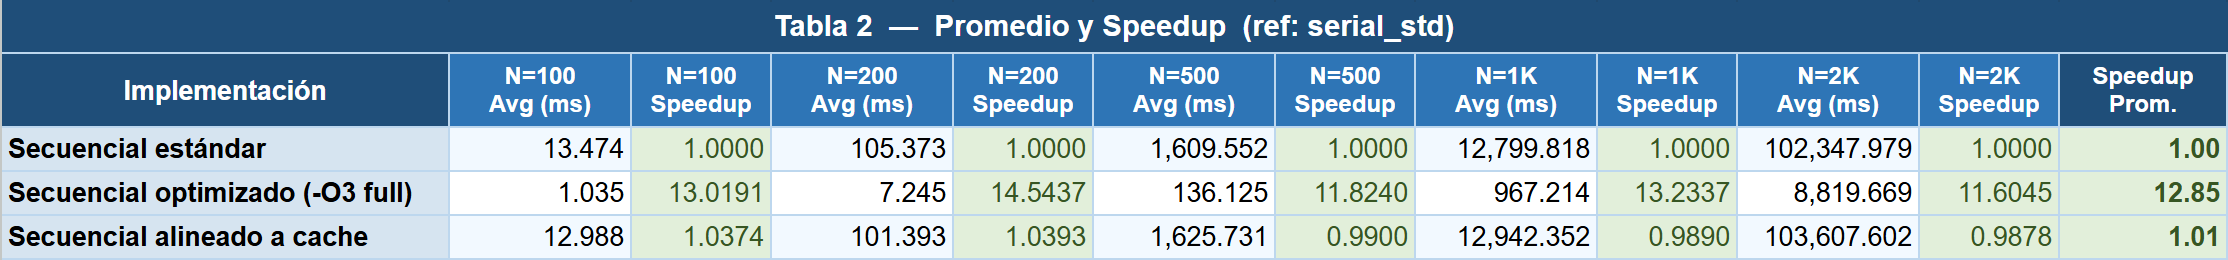
\includegraphics[width=1\textwidth]{images/tables/serial_speedup.png}
   \caption{Speedup del algoritmo secuencial optimizado por cache line}
   \label{tab:cache_speedup}
\end{table}

\begin{figure}[H]
   \centering
   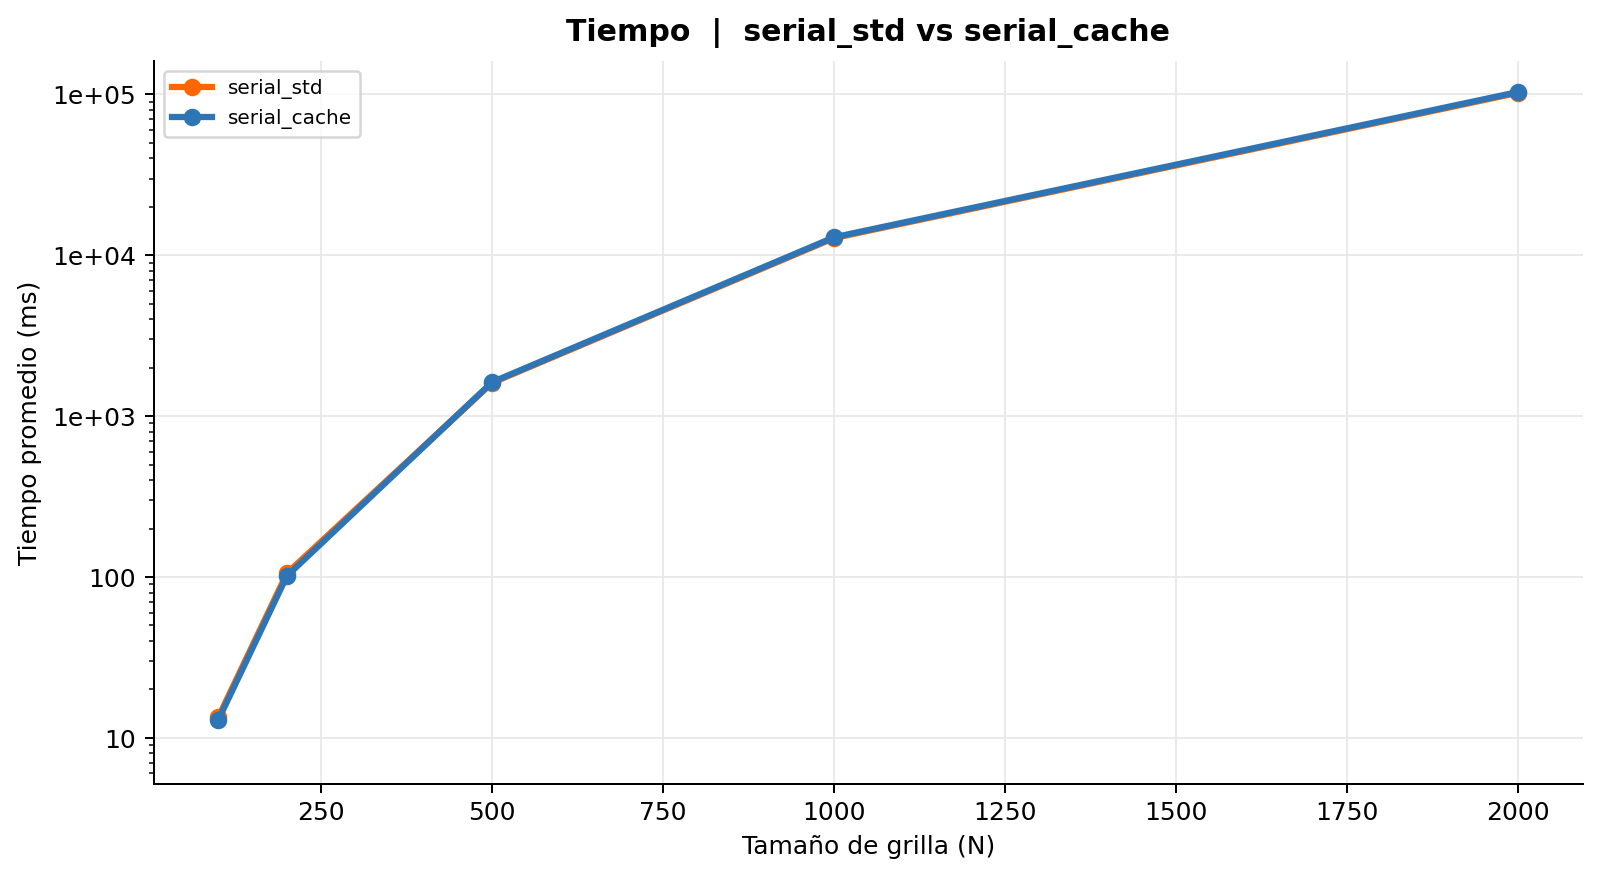
\includegraphics[width=1\textwidth]{images/charts/cache_time.png}
   \caption{Comparación del tiempo de ejecución entre el algoritmo secuencial y el algoritmo secuencial optimizado por cache line}
   \label{fig:chart_cache_time}
\end{figure}

\begin{figure}[H]
   \centering
   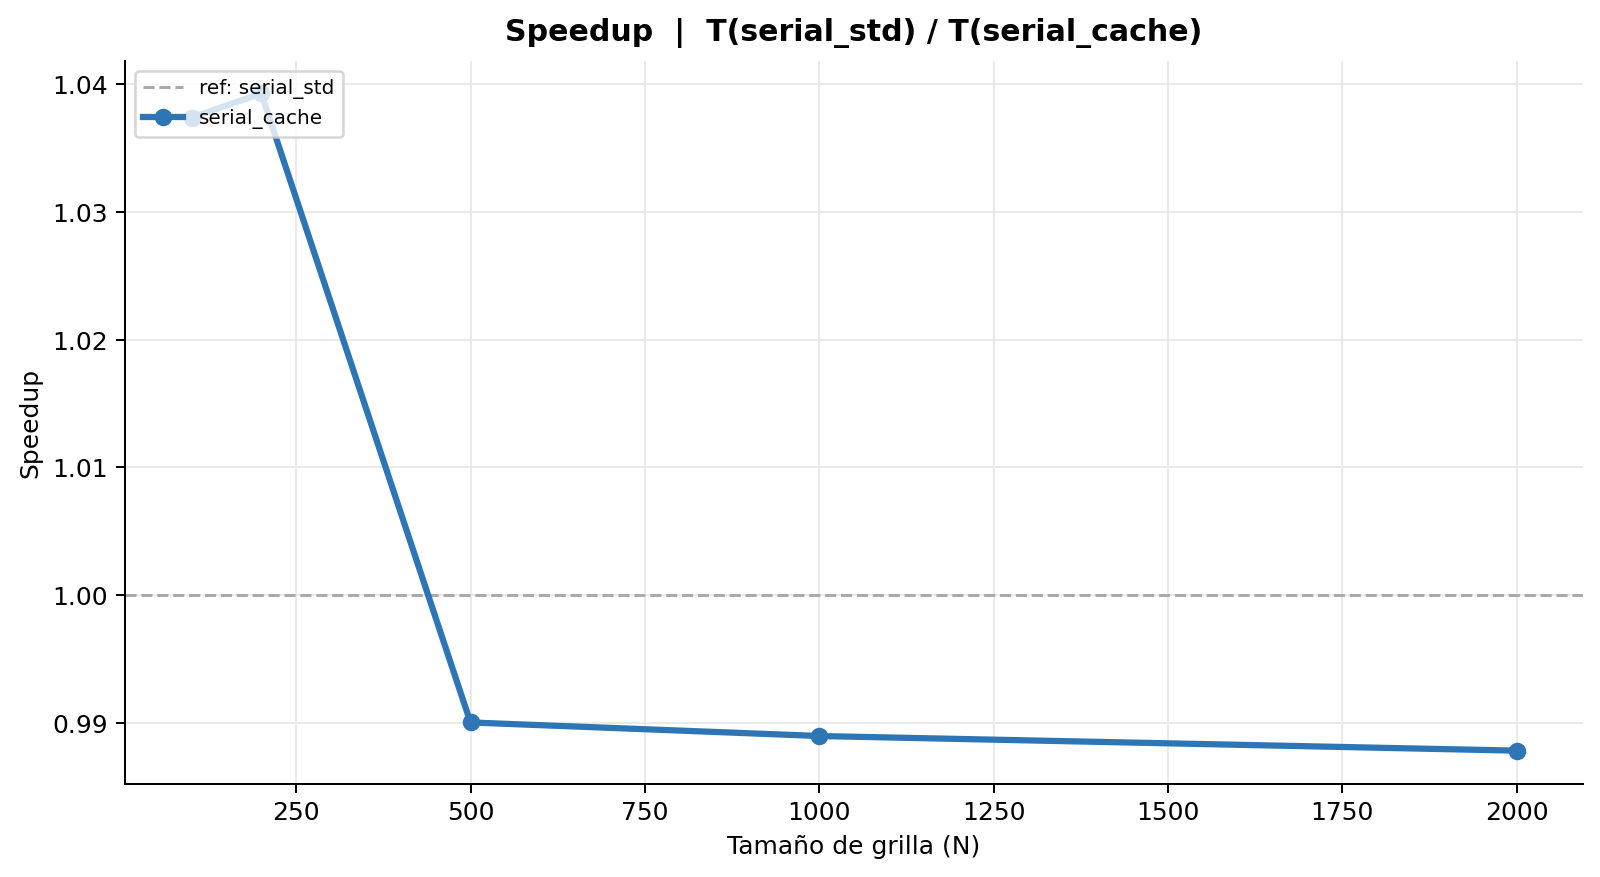
\includegraphics[width=1\textwidth]{images/charts/cache_sp.png}
   \caption{Comparación del speedup entre el algoritmo secuencial y el algoritmo secuencial optimizado por cache line}
   \label{fig:chart_cache_speedup}
\end{figure}


%================================
\subsection{Resultados de las pruebas del algoritmo optimizado por compilador}
\label{sec:Resultados_compilador}

Para este algoritmo se usaron las siguientes opciones de compilación: -O3, -funroll-loops, -fomit-frame-pointer y -march=native. Estas opciones permiten al compilador realizar optimizaciones agresivas, como la eliminación de código innecesario, el desenrollado de bucles y la generación de código específico para la arquitectura del procesador. Estas optimizaciones pueden mejorar significativamente el rendimiento del algoritmo, especialmente en casos donde se realizan muchas iteraciones o se manejan grandes cantidades de datos. 

El signigicado de cada bandera es el siguiente:
\begin{itemize}
   \item \textbf{-O3:} Esta bandera habilita un nivel de optimización agresivo, permitiendo al compilador aplicar una amplia gama de técnicas para mejorar el rendimiento del código.
   \item \textbf{-Wall:} Activa la mayoría de las advertencias del compilador, lo que ayuda a identificar posibles problemas en el código que podrían afectar su rendimiento o funcionalidad.
   \item \textbf{-march=native:} Permite al compilador generar código optimizado para la arquitectura específica del procesador en el que se está compilando, aprovechando las características y capacidades de hardware disponibles.
   \item \textbf{-funroll-loops:} Habilita el desenrollado de bucles, lo que puede mejorar el rendimiento al reducir la sobrecarga de control de bucle y aumentar la paralelización de las instrucciones.
   \item \textbf{-flto:} Habilita la optimización a nivel de enlace, lo que permite al compilador realizar optimizaciones globales en todo el programa, incluso entre diferentes archivos de código fuente.
   \item \textbf{-ffast-math:} Permite al compilador realizar optimizaciones agresivas en operaciones matemáticas, lo que puede mejorar el rendimiento a costa de la precisión en algunos casos como la evaluación de funciones trigonométricas.
   \item \textbf{-fomit-frame-pointer:} Indica al compilador que no utilice un puntero de marco para las funciones, es decir, que no cree un marco de pila para cada función, lo que puede mejorar el rendimiento al reducir la cantidad de instrucciones necesarias para gestionar la pila de llamadas.
\end{itemize}


Se realizaron las pruebas para el algoritmo secuencia optimizado por compilador y estos fueron los resultados obtenidos:

\begin{table}
   \centering
   
\includegraphics[width=1\textwidth]{images/tables/compiler_time.png}
   \caption{Resultados del algoritmo secuencial optimizado por compilador}
   \label{tab:compiler}
\end{table}

\begin{table}[H]
   \centering
   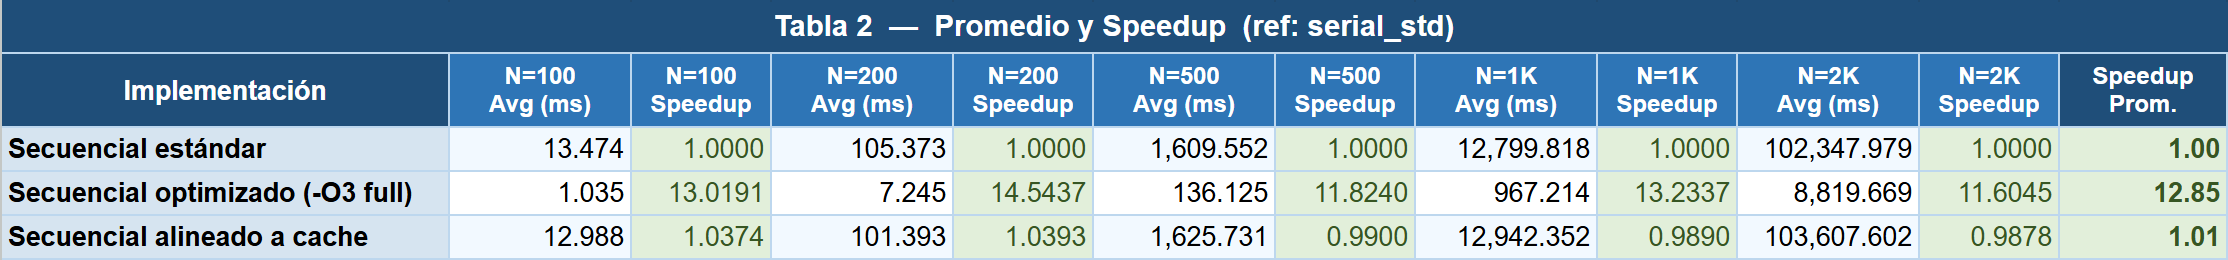
\includegraphics[width=1\textwidth]{images/tables/serial_speedup.png}
   \caption{Speedup del algoritmo secuencial optimizado por compilador}
   \label{tab:compiler_speedup}
\end{table}


\begin{table}[H]
   \centering
   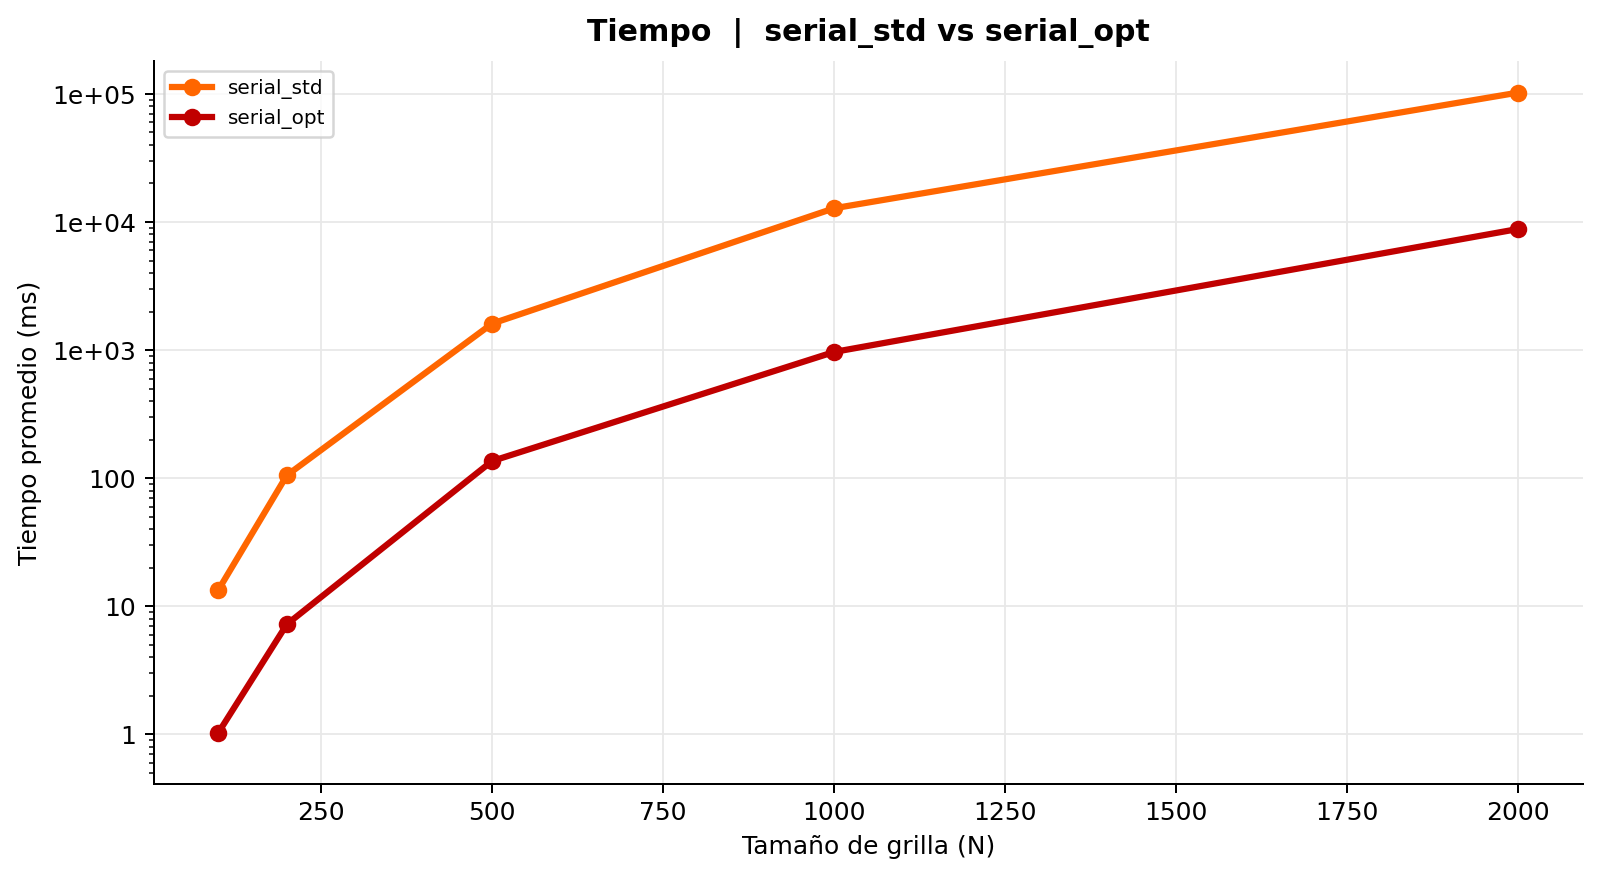
\includegraphics[width=1\textwidth]{images/charts/compiler_time.png}
   \caption{Comparación del tiempo de ejecución entre el algoritmo secuencial y el algoritmo secuencial optimizado por compilador}
   \label{tab:compiler_time}
\end{table}

\begin{figure}[H]
   \centering
   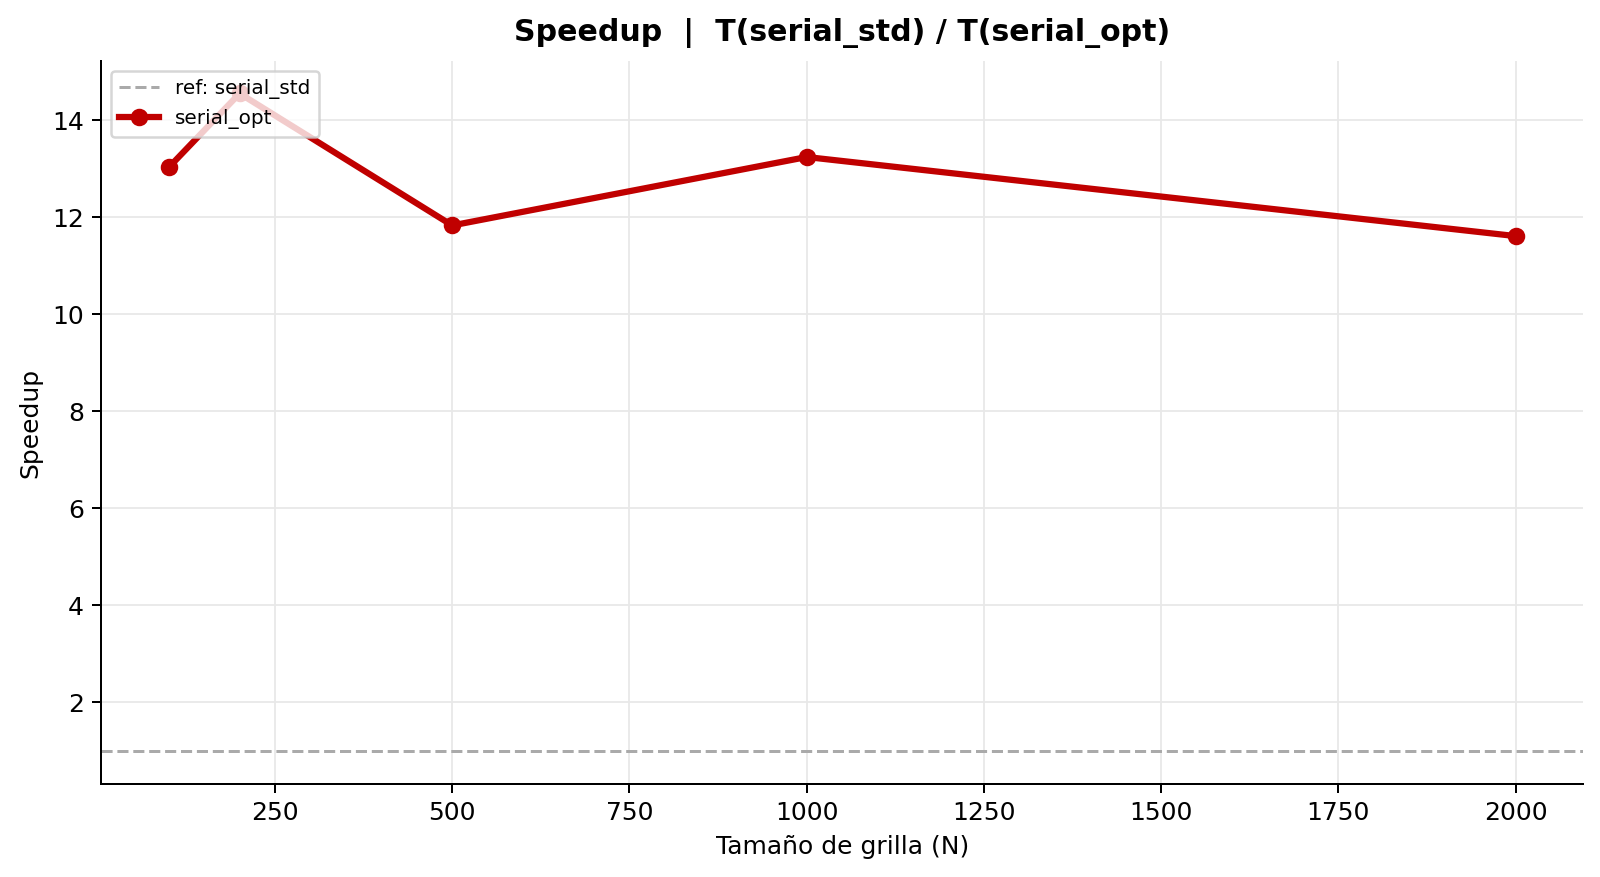
\includegraphics[width=1\textwidth]{images/charts/compiler_sp.png}
   \caption{Comparación del speedup entre el algoritmo secuencial y el algoritmo secuencial optimizado por compilador}
   \label{fig:chart_compiler_speedup}
\end{figure}


%================================
\subsection{Resultados del algoritmo paralelizado con hilos}
\label{sec:Resultados_hilos}

Para esta implementación se utilizó la biblioteca de hilos POSIX (pthreads) para crear múltiples hilos que ejecutan el algoritmo de Jacobi en paralelo. Cada hilo se encarga de procesar una parte del arreglo, lo que permite aprovechar la capacidad de procesamiento de múltiples núcleos del CPU. Se realizaron pruebas con diferentes números de hilos (2, 4, 6, 8 y 12) para evaluar el impacto en el rendimiento. Estos fueron los resultados obtenidos:

\begin{table}
   \centering
   
\includegraphics{images/tables/threads_time.png}
   \caption{Resultados del algoritmo paralelizado con hilos}
   \label{tab:threads}
\end{table}

\begin{table}[H]
   \centering
   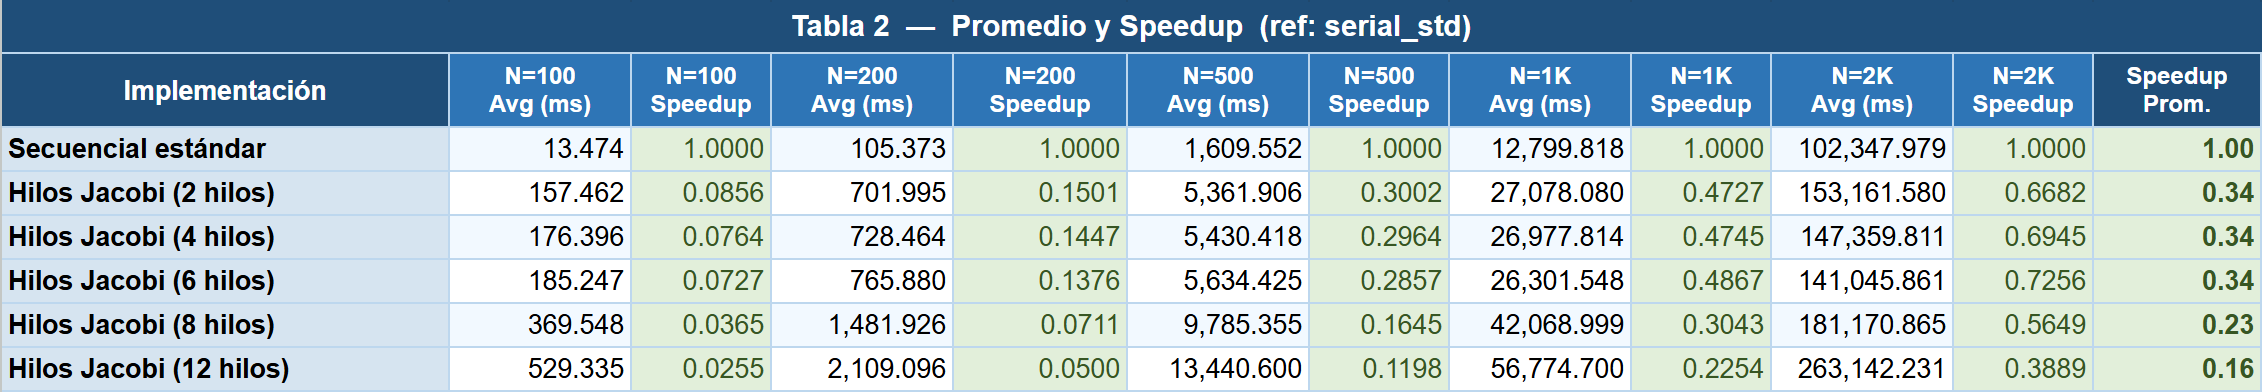
\includegraphics[width=1\textwidth]{images/tables/threads_speedup.png}
   \caption{Speedup del algoritmo paralelizado con hilos}
   \label{tab:threads_speedup}
\end{table}

\begin{figure}[H]
   \centering
   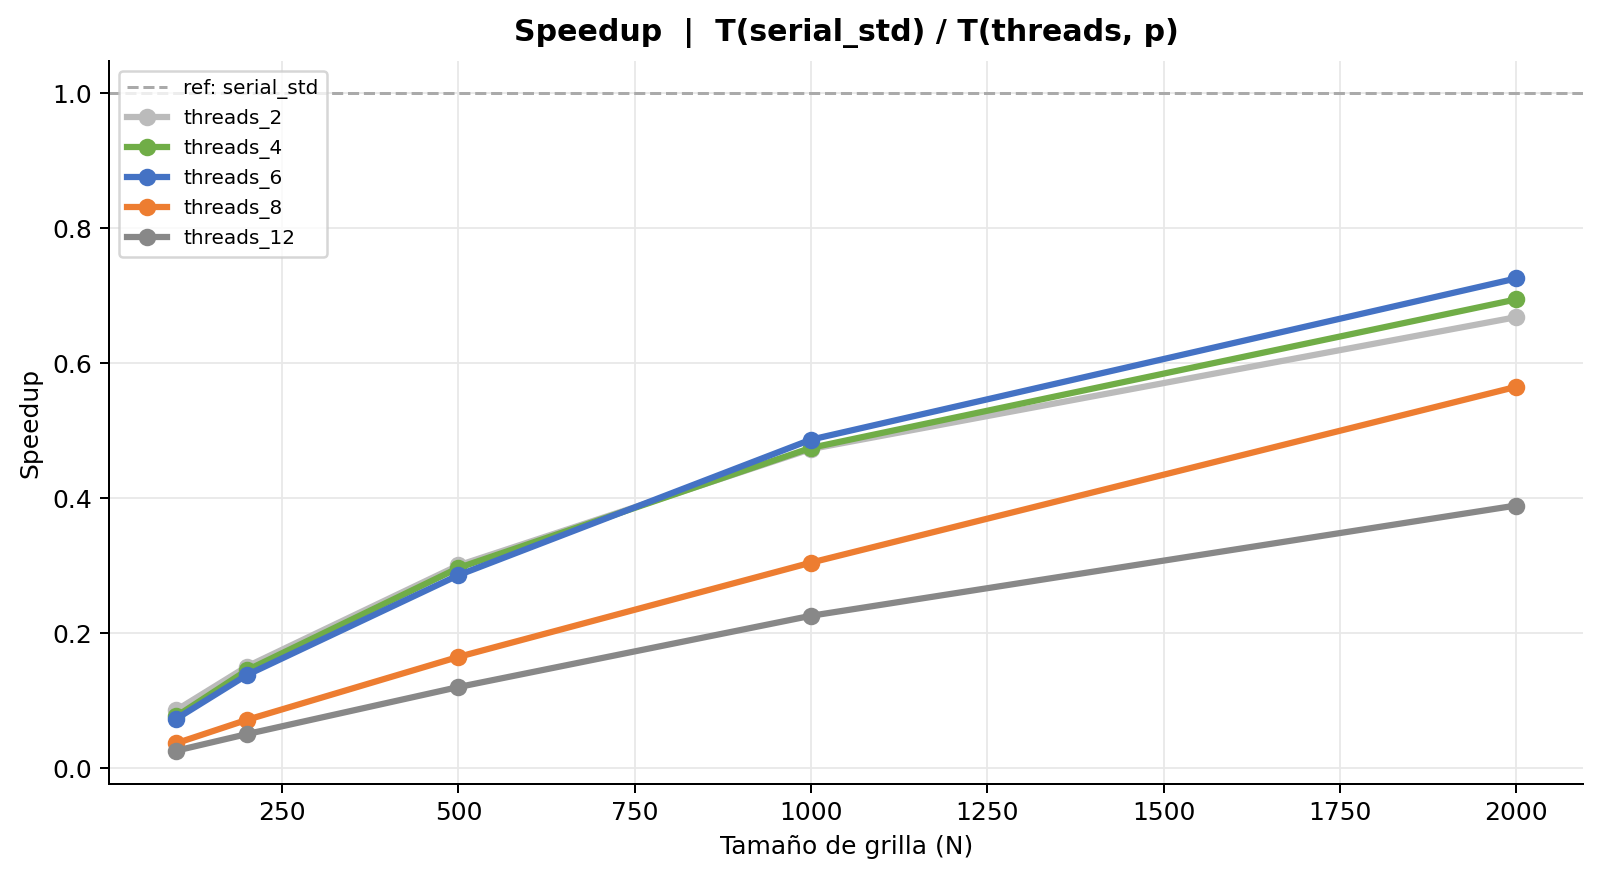
\includegraphics[width=1\textwidth]{images/charts/threads_sp.png}
   \caption{Comparación del speedup entre el algoritmo secuencial y el algoritmo paralelizado con hilos}
   \label{fig:chart_threads_speedup}
\end{figure}


%================================
\subsection{Resultados del algoritmo paralelizado por procesos}
\label{sec:Resultados_procesos}

Para esta implementación se utilizó la biblioteca de procesos POSIX (fork) para crear múltiples procesos que ejecutan el algoritmo de Jacobi en paralelo. Cada proceso se encarga de procesar una parte del arreglo, lo que permite aprovechar la capacidad de procesamiento de múltiples núcleos del CPU. Se realizaron pruebas con diferentes números de procesos (2, 4, 6, 8 y 12) alienados a las pruebas con hilos realizadas para evaluar el impacto en el rendimiento. Estos fueron los resultados obtenidos:

\begin{table}
   \centering
   
\includegraphics{images/tables/processes_time.png}
   \caption{Resultados del algoritmo paralelizado por procesos}
   \label{tab:processes}
\end{table}

\begin{table}
   \centering
   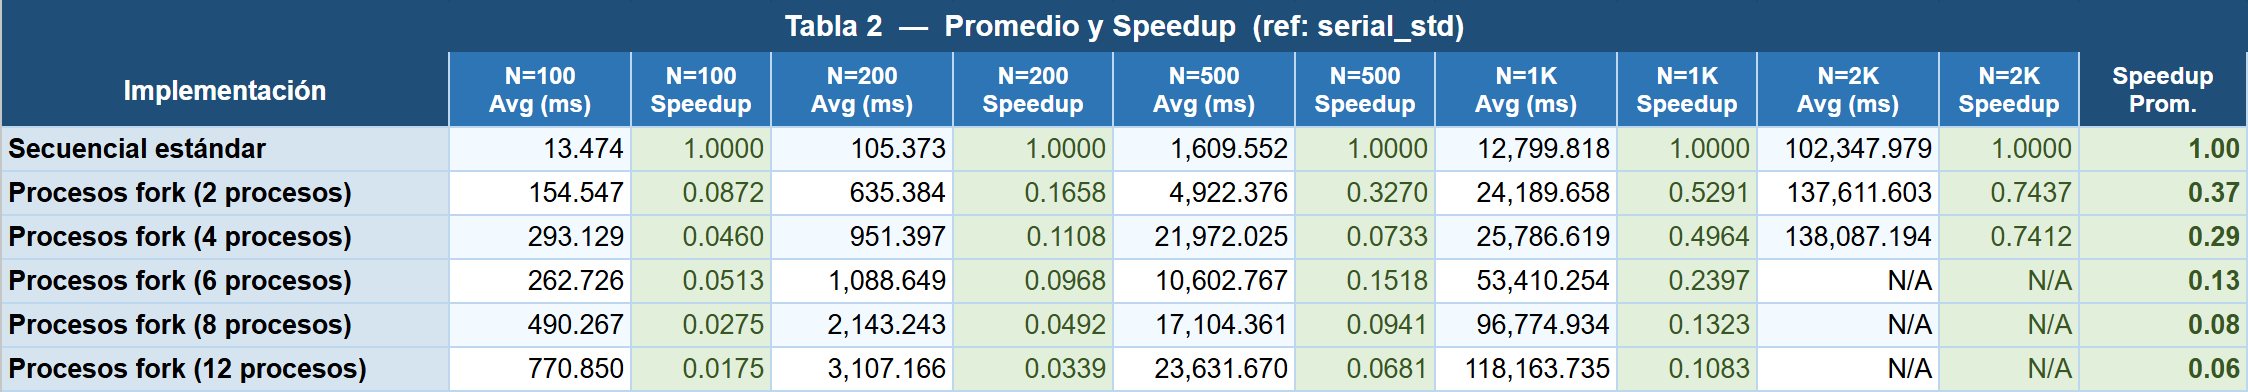
\includegraphics[width=1\textwidth]{images/tables/processes_speedup.png}
   \caption{Speedup del algoritmo paralelizado por procesos}
   \label{tab:processes_speedup}
\end{table}

\begin{figure}
   \centering
   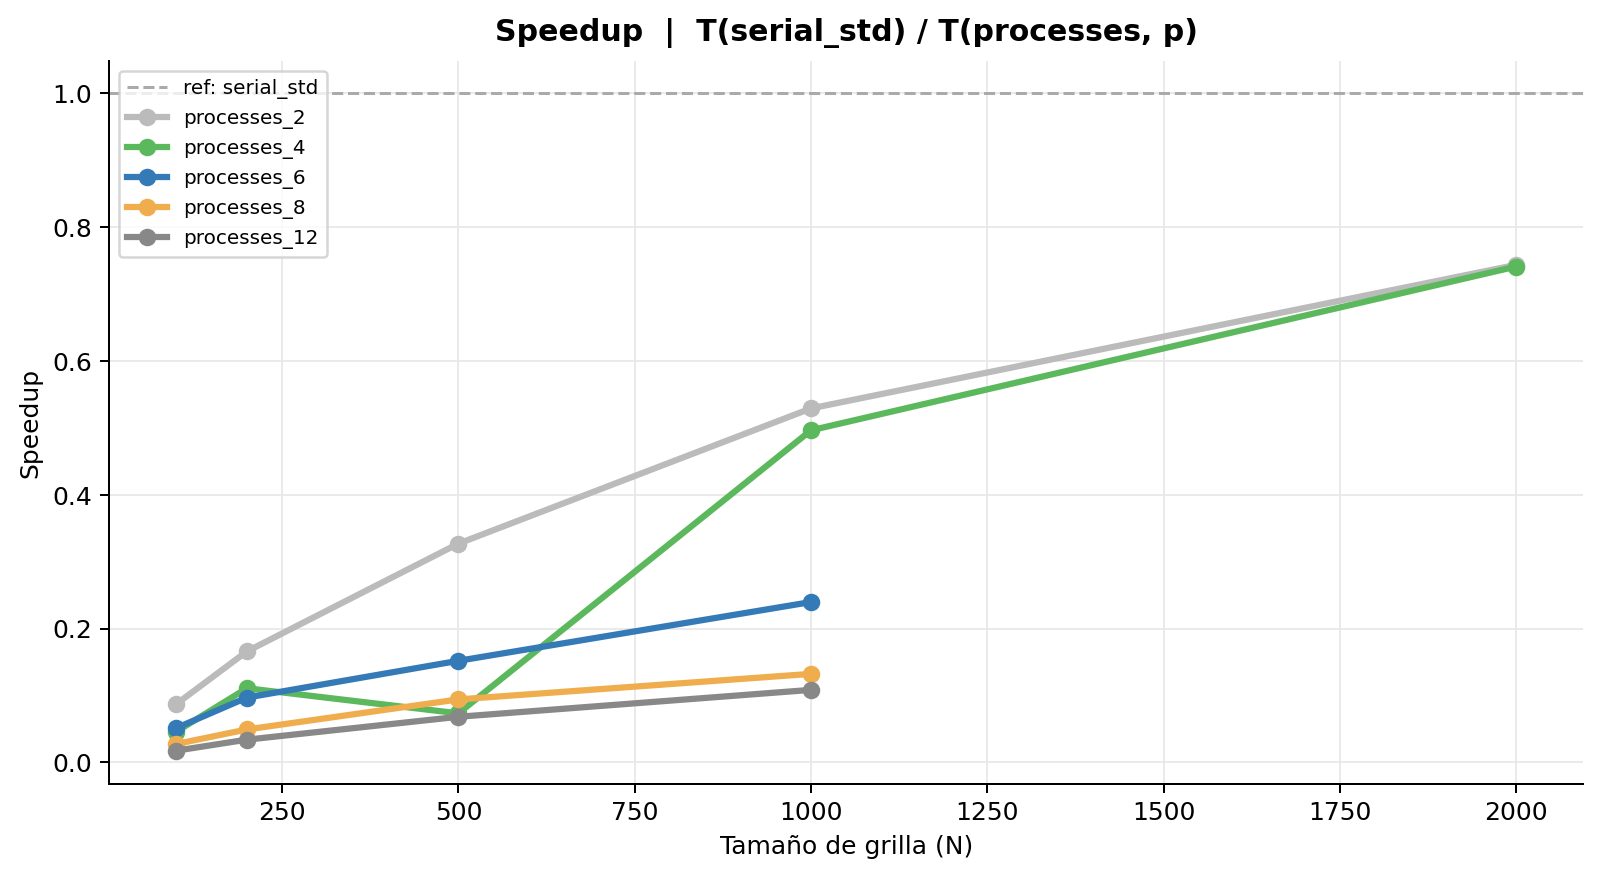
\includegraphics[width=1\textwidth]{images/charts/processes_sp.png}
   \caption{Comparación del speedup entre el algoritmo secuencial y el algoritmo paralelizado por procesos}
   \label{fig:chart_processes_speedup}
\end{figure}
